Our simulation consists of a set of agents that try to navigate a randomly
generated maze, these agents are meant to simulate robots in the real world. 
They communicate with a set agents that act as soft bots in web services. These
soft bots support the robots in accomplishing their task to rescue people from
the maze. For communication between the agents we use the SPADE \footnote{https://pypi.python.org/pypi/SPADE} framework as our top layer.

\subsection{Simulation Model}
The simulation consists of two web services, two types of robots and a
supervisor. The web services are a data store and a path planner. The data
store is used to store the map, while the path planner can be given a map, a
starting point and a target location. The robots can either be a search robot,
they can sense the environment; or they can be rescuers in which case they have
actuators and the capability to carry victims. The search bots explore the maze
with help from the supervisor, while the rescue bots are sent into the maze to
collect the targets. The supervisor is the link between all these components.
It also keeps track of the parts of the map that have been visited and the
areas of the map that have unexplored corridors. The supervisor also makes sure
that the search bots are not all at the some location but explore different
parts of the map.

\subsubsection{Data Store agent}
The data store agent represents a web service that allows you to store raw data in our database. It can be updated and queried like a regular database.  

\subsubsection{Path planner agent}
The path planner represents a web service that uses the A* algorithm
\cite{astar} to plan a route through a grid based maze, such as
\cite{astarweb}. The pseudocode for A* is shown in \autoref{fig:pseudocode} .

\begin{figure}[h]
	\centering
		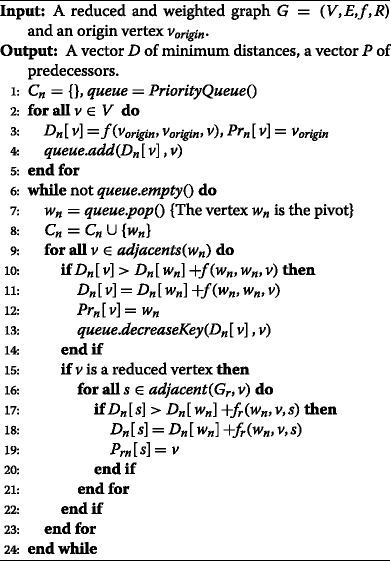
\includegraphics[width=6cm]{Astar}
	\caption{A* pseudocode}
	\label{fig:pseudocode}
\end{figure}

\subsubsection{Search robot agents}
The search bots are robots that are simple platforms with some sensors. They
can be thought of as the eyes of the system, these agents are also able to move
around the maze quickly. This makes them ideal for searching through buildings.
They travel through the maze along the straight corridors until they reach a
fork in the maze. Then they call upon the supervisor to give them a new target
to travel to and explore. If they get stuck in a dead end they will request a
new search location from the supervisor. They will then ask the path planning
service to return a route to get to the new search location.

\subsubsection{Supervisor agent}
The Supervisor is the central part of the system that makes sure that all
the components work together. It manages most of the resources and it keeps
track of where robots are. It also directs all the search robots and to make
sure that they don't all try to explore the same area.

\subsubsection{Interaction}
Every time a search agent uncovers a new location, it will send a message to
the data store so it can be updated with the additional data. This information
can later be retrieved.

When a search bot gets stuck, it reports its current location to the
supervisor. The supervisor then requests the current map. Then it sends the
map, the location of the stuck searcher and a position that has not been
visited yet to the path planner. The planner will return a path if it is
possible. The supervisor then sends this path to the searcher so it can
resume exploring.

\subsection{Experimental design}
The supervisor is an important link in our system, and we would want it to
be as robust as possible. Therefore we would want to know whether the
system performs better if the supervisor is one monolithic object or if
there is division of labour between the agents. For this we implement
multiple structures for the supervisor, one where the supervisor is a central
director orchestrating all agents and one where all agents are working together.

Because the performance is also dependent on the number of search agents, this
number will also be varied. This will give us a clear overview of the
different strategies and the interaction with the number of agents.

The definition for better is the time it took to rescue the targets.  The
time will be measured from the start of the simulation until the moment that
all targets are returned to the start and the entire maze is explored. The last
condition is included because the system does not know whether all targets
are recovered until the entire maze has been explored. Because the maze is
randomly generated, the simulation will be ran several times for each
combination of supervisor and number of searchers.


\begin{figure}[h]
	\centering
		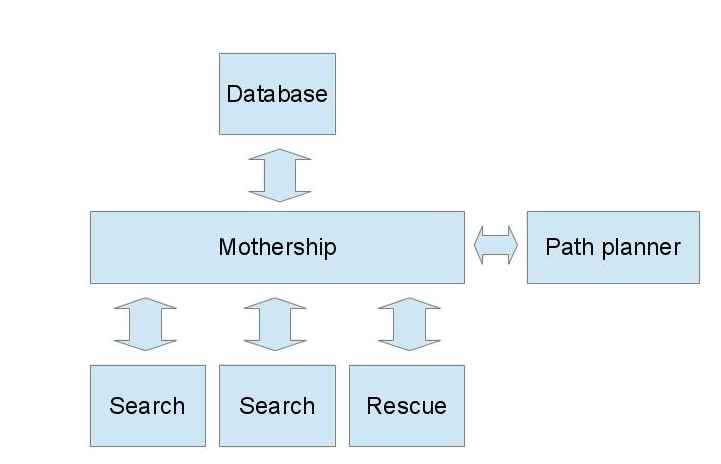
\includegraphics[width=6cm]{mothership}
	\caption{Mothership overview}
	\label{fig:mothership}
\end{figure}

\begin{figure}[h]
	\centering
		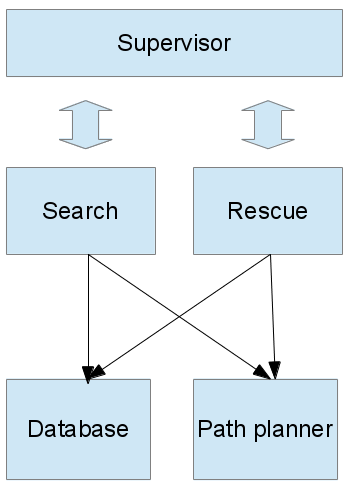
\includegraphics[width=6cm]{supervisor}
	\caption{Supervisor overview}
	\label{fig:supervisor}
\end{figure}
